\documentclass{article}
\usepackage[margin=1in,a4paper]{geometry}
\usepackage[utf8]{inputenc}
\usepackage[cyr]{aeguill}
\usepackage[francais]{babel}
\usepackage{hyperref}
\usepackage{amsmath}
\usepackage{gensymb}
\usepackage{enumitem,amssymb}
\newlist{checks}{itemize}{2}
\setlist[checks]{label=$\square$}
\usepackage{graphicx}
\usepackage{amsthm}
\usepackage{amsfonts}
\usepackage{multicol}
\usepackage{pgfplots}
\pgfplotsset{compat=newest}
\usetikzlibrary{calc}
\usepackage{mathtools}
\usepackage{array}
\usepackage[T1]{fontenc}
\usepackage{lmodern}
\usepackage{tabularx}
\usepackage{fancyhdr}
\usepackage{pst-func}
\usepackage{xcolor}
\usepackage{nicefrac}
\usepackage{mdframed}
\usepackage[boxed,vlined]{algorithm2e}
\usepackage{cleveref}
\newcommand{\Lim}[1]{\raisebox{0.5ex}{\scalebox{1}{$\displaystyle \lim_{#1}\;$}}}
\usepackage{float}
%\usepackage[top=2.5cm, bottom=2cm, left=2cm, right=2cm, showframe]{geometry}
\usepackage[top=2.5cm, bottom=2cm, left=2cm, right=2cm]{geometry}
\newcommand{\N}{\mathbb{N}}
\newcommand{\R}{\mathbb{R}}
\renewcommand{\C}{\mathbb{C}}
\renewcommand{\P}{\mathbb{P}}
\newcommand{\w}{\omega}
\newcommand{\p}{\partial}
\newcommand{\cross}{\times}
\newcommand{\Col}{\text{Col}}
\newcommand{\Tr}{\text{Tr}}
\newcommand{\bigzero}{\makebox(0,0){\text{\huge0}}}
\DeclareMathOperator{\Ima}{Im}
\DeclareMathOperator{\Vect}{Vect}
\usepackage{mathtools, stmaryrd}
\usepackage{xparse} \DeclarePairedDelimiterX{\Iintv}[1]{\llbracket}{\rrbracket}{\iintvargs{#1}}
\NewDocumentCommand{\iintvargs}{>{\SplitArgument{1}{,}}m}
{\iintvargsaux#1} %
\NewDocumentCommand{\iintvargsaux}{mm} {#1\mkern1.5mu..\mkern1.5mu#2}
\newcommand{\Cc}{{\mathbb{C}}}
\newcommand{\Ct}{\Cc^\times}
\newcommand{\Hh}{{\mathbb{H}}}
\newcommand{\Nn}{{\mathbb{N}}}
\newcommand{\Zz}{{\mathbb{Z}}}
\newcommand{\Zzn}{\Zz/n\Zz}
\newcommand{\ZzNt}{(\Zz/N\Zz)^\times}%quotient 
\newcommand{\Rr}{{\mathbb{R}}}
\newcommand{\Rt}{{\Rr^\times}}
\newcommand{\Qt}{{\Qq^\times}}
\newcommand{\Qq}{{\mathbb{Q}}}
% Custom titling
\usepackage{titling}
\usepackage{tcolorbox}

\title{\textbf{Analyse Avancée -- Corrigé 1}}

\renewcommand{\maketitlehookb}{
\begin{center}

\includegraphics[width=2cm]{Cours/assets/imgs/logo-round.png}
\end{center}
}

\author{Students 4 Students}
\date{Septembre 2022}

% Exercises environment and styling
\usepackage{amsthm}
\newtheoremstyle{exercice}%
    {3pt}% Space above
    {3pt}% Space below
    {\large}% Body font
    {}% Indent amount
    {\bfseries}% Theorem head font
    {}% Punctuation after theorem heading
    {\newline}% Space after theorem heading
    {\thmname{#1}\thmnumber{ #2}\thmnote{: #3}}% Theorem head spec (can be left empty, meaning ‘normal’)
\theoremstyle{exercice}
\newtheorem{exercice}{Exercice}


\begin{document}

% Header
\pagestyle{fancy}
\fancyhead[L]{Students 4 Students}
\fancyhead[C]{\textit{Analyse avancée - Corrigé 1}}
\fancyhead[R]{Septembre 2022}

\maketitle

\begin{exercice}
    
Faisons la preuve par contraposition, donc montrons que si $a$ est impair alors $a^2$ est impair.\\

Soit $a=2k+1$, $k\in \Zz$, un nombre impair. Alors $a^2=(2k+1)^2=2\cdot(2k^2+2k)+1=2n+1$ avec $n=2k^2+2k\in \Zz$. Donc $a^2$ est bien impair. La proposition est donc démontrée par contraposition.$~~\Box$


\end{exercice}

\begin{exercice}
Les réponses sont les suivantes:

\begin{enumerate}
    \item $\{0,3,4,7,8,9\}$
    \item \{ 3 \}
    \item   (0, 2]
    \item (0.5, 1]
    \item  \O
    \item \{4,8,3\}$\cup$[0,1]
\end{enumerate}

\end{exercice}



\begin{exercice}
    Commençons par la suite arithmétique. Montrons que $x_n=x_0+n\cdot r$ par récurrence.

La condition est trivialement vérifiée pour $n=0$. Passons à l'hérédité donc supposons que la condition est vraie pour $n$, montrons qu'elle est vraie pour $n+1$. On a :

\begin{equation}
    x_{n+1}=x_n+r=x_0+n\cdot r+r=x_0+(n+1)\cdot r,
\end{equation}
en ayant utilisé l'hypothèse de récurrence. La propriété est donc démontrée.\\

Puis pour la suite géométrique, montrons que $x_n=x_0\cdot r^n$ par récurrence.

La condition est trivialement vérifiée pour $n=0$. Passons à l'hérédité donc supposons que la condition est vraie pour $n$, montrons qu'elle est vraie pour $n+1$. On a :

\begin{equation}
    x_{n+1}=x_n\cdot r=(x_0\cdot r^n)\cdot r=x_0\cdot r^{n+1},
\end{equation}
en ayant utilisé l'hypothèse de récurrence. La propriété est donc démontrée.



\end{exercice}

\begin{exercice}[Convergence de suite, suite monotone bornée]\\
    
$~~~$ \textbf{Méthode 1: Par la définition}\\

\textbf{a)} \\

\begin{figure}[H]
    \centering
    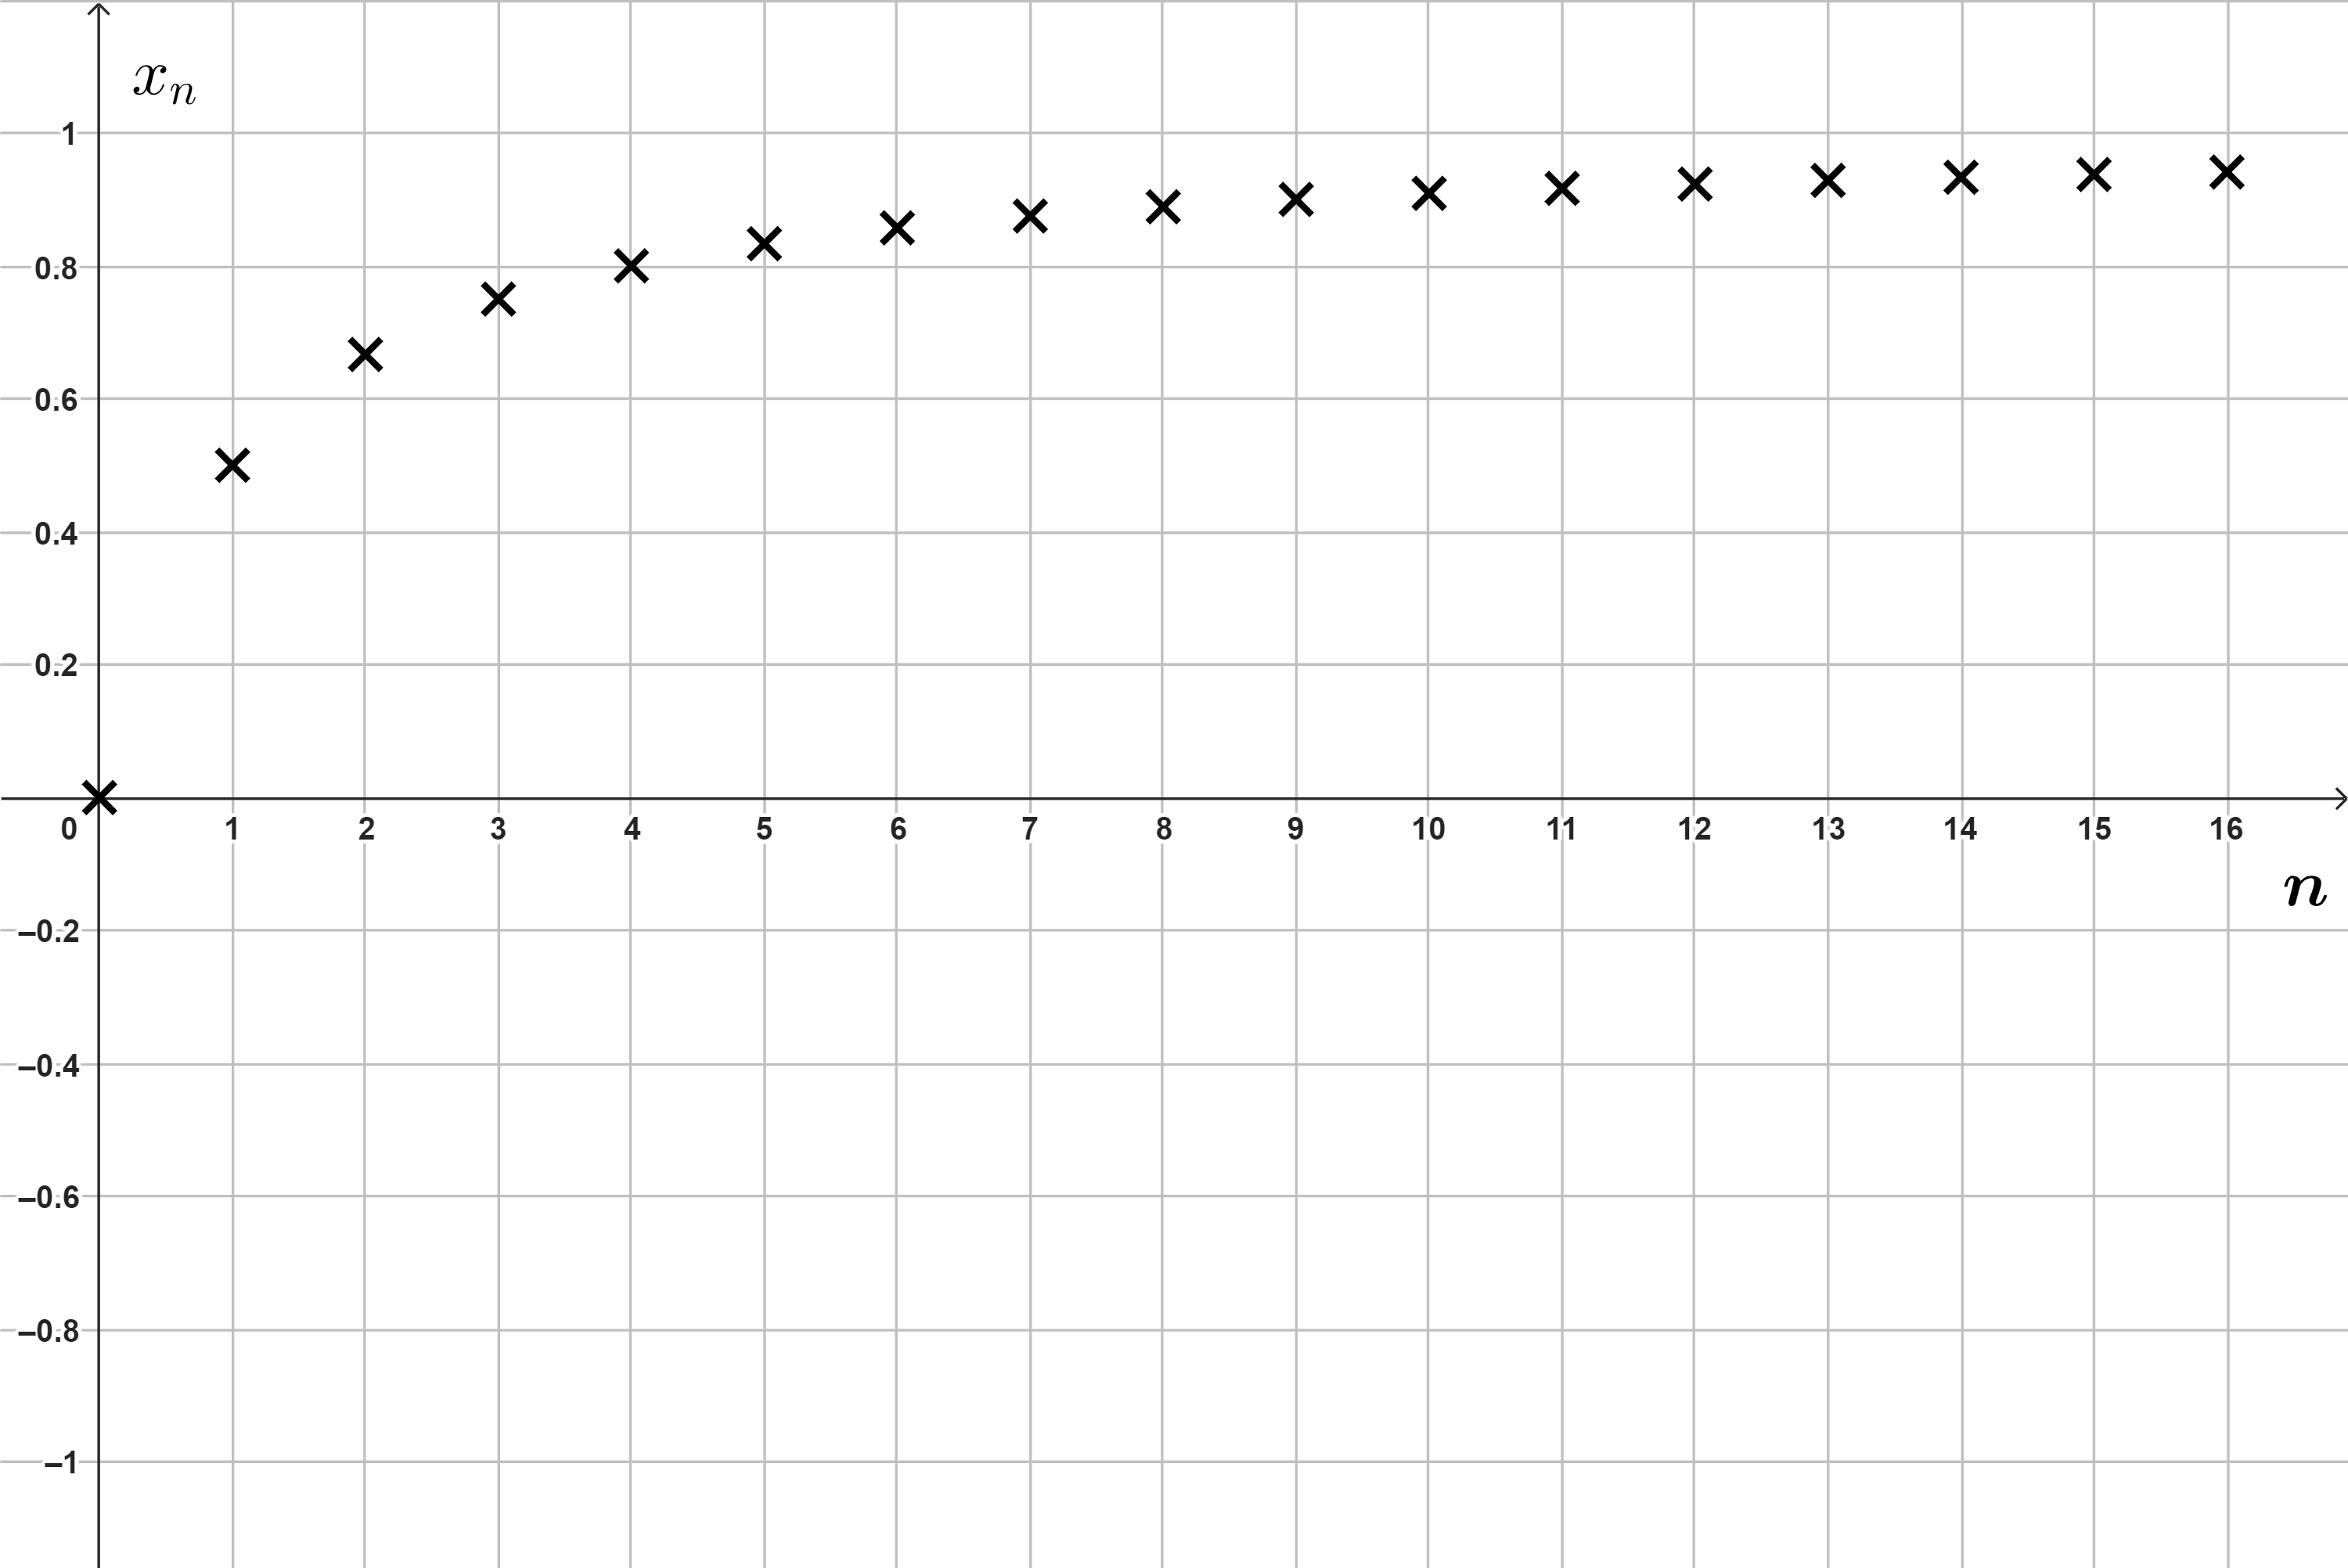
\includegraphics[scale=0.7]{Exercices/schema1.png}
    \caption{Representation des premiers termes de la suite $x_n=\frac{n}{n+1}$.}
    \label{fig:enter-label}
\end{figure}

\textbf{b)} La suite converge vers 1. \\

\textbf{c)} $N = 10$, car pour $n = 10$ on a $x_n =  \frac{10}{11}$, soit un écart avec la limite de 1 qui vaut $\frac{1}{11}$, ce qui est bien \textit{strictement} inférieur à 0.1.\\

\textbf{d)} L'écart entre la limite de 1 et la suite doit être inférieur à $\epsilon$, soit:
\begin{equation}
    \Bigl\lvert 1-\frac{n}{n+1}\Bigl\rvert < \epsilon \iff \frac{1}{n+1} < \epsilon \iff \frac{1-\varepsilon}{\varepsilon}<n.
\end{equation}
Notez qu'on se ``débarasse" de la valeur absolue car son argument est toujours positif. \\

\faLightbulbO \quad \fbox{\textbf{Discutez}} 
La suite diverge, donc au lieu d'utiliser la définition de limite de suite convergente (avec $|x_n - l| < \epsilon$) on utilise celle de limite infinie (avec $x_n \geq M$, car la limite est de $+ \infty$).\\

\textbf{Méthode 2: Par le théorème des suites monotones bornées}\\

\textbf{a)} On peut par exemple borner la suite par 1: 
\begin{equation}
    \frac{n}{n+1} < 1 \iff n < n+1 \iff 0 < 1.
\end{equation}
Le suprémum de la suite est 1 (c'est le plus petit majorant de la suite - on l'a prouvé indirectement à l'exercice précédent en montrant que la suite convergeait vers 1). Ce suprémum n'étant jamais atteint, ce n'est pas un maximum. Noter que cette démonstration consiste à n'utiliser que des équivalences pour tomber sur quelque chose d'évident et après remonter la démonstration. Autrement dit, nous aurions pu partir de $0<1$ et aller jusqu'à la borne de notre suite.\\

\textbf{b)} Une manière de procéder consiste à tout simplement utiliser la définition de suite croissante: $x_n \leq x_{n+1}$, soit:
\begin{equation}
    \frac{n}{n+1} \leq \frac{n+1}{n+2} \iff n^2 + 2n \leq n^2 + 2n + 1 \iff 0 \leq 1.
\end{equation}
où la deuxième expression est obtenue en mettant les deux fractions au même dénominateur $(n+1)(n+2)$, puis en multipliant les deux membres de l'inéquation par ce dénominateur positif (donc pas d'inversion de l'inégalité).
\\

\textbf{c)} Toute suite bornée supérieurement a un suprémum $b$, qui peut être défini comme suit:
\begin{equation}
    \forall \epsilon, \exists \ ñ \quad tel \ que \quad b-\epsilon \leq x_{ñ} \leq b.
\end{equation}
En combinant avec la définition de croissance on obtient:
\begin{equation}
    \forall \epsilon, \exists \ ñ \quad tel \ que \quad b-\epsilon \leq x_{ñ} \leq x_{ñ+1} \leq ... \leq b,
\end{equation}
et ainsi $ \lim_{x\to\infty} x_n = b = sup\{x_n; \ n \in \Nn\}$.
\\

\faLightbulbO \quad \fbox{\textbf{Discutez}} L'astuce est de commencer par trouver la valeur de la limite de cette suite récurrente. A sa limite, cette suite est censée stagner, soit, en prenant $l$ la limite:
\begin{equation}
    l = \frac{l + 1}{2},
\end{equation}
ce qu'on appelle un point fixe.\\
En résolvant cette équation du premier degré, on trouve que la limite, si elle existe, doit être de 1. Le point initial $x_0$ de la suite étant inférieur à 1, il faudrait que la suite soit croissante bornée supérieurement pour utiliser le théorème des suites monotones bornées (car 0.5 est plus petit que 1).\\
Commençons par montrer par récurrence qu'elle est bornée supérieurement par 1. Le premier terme $x_0 = 0.5$ est bien plus petit que 1. Il reste à montrer que $x_n \leq 1 \Rightarrow x_{n+1} \leq 1$.
\begin{equation}
    x_n \leq 1 \Rightarrow x_n + 1 \leq 2 \Rightarrow \frac{x_n + 1}{2} = x_{n+1} \leq 1.
\end{equation}
Enfin, montrons que pour $x_n \leq 1$, la suite est croissante, soit $x_n \leq x_{n+1}$:
\begin{equation}
    x_n \leq x_{n+1} = \frac{x_n + 1}{2} \iff 2x_n \leq x_n + 1 \iff x_n \leq 1.
\end{equation}


\end{exercice}

\end{document}